\chapter{Técnicas de reconstrução baseadas em \emph{Time Of Flight}}\label{cap:kinect}
%======================================================================================

\section*{Introdução}

\emph{Time of Flight}~\cite{gokturk2004time} ou Tempo de Vôo é um \textbf{método ótico ativo}, que consegue determinar a localização de objetos no alcance do sensor de infra-vermelho (no caso do Kinect, um sensor ToF invisível), a partir de alterações na matriz do projetor de feixes de infra-vermelho (\eg, Kinect versão 1~\cite{smisek20133d}). Existe também, um outro método que utiliza fótons, que viajam na velocidade da luz. Onde o valor resultante cálculo da diferença da emissão e da chegada dos fótons aos detectores é utilizado na criação de uma probabilidade de distribuição localizando o evento detectado a uma distância do eixo do escaneador (\eg, Kinect versão 2~\cite{lachat2015first,valgma20163d}). 

\section{Kinect}

\subsection*{Introdução}

Um componente criado pela Microsoft para fins recreativos (como no XBox, por
exemplo), se tornou uma das mais conhecidas ferramentas de reconstrução 3D no
cenário atual. Sua primeira versão (Kinect V1)~\ref{fig:kinectv1} utiliza uma técnica similar à empregada no projeto da Universidade de Stanford, com luz estruturada, porém, diferentemente dos escaners a \emph{laser}, o Kinect tem um custo monetário baixo e é acessível a todo público em geral (desde entusiastas e amadores até profissionais da área). 

O Kinect V2 é composto de uma câmera RGB-D (\emph{Red, Green, Blue} e \emph{Depth}) e utiliza uma projeção de fótons, é mais robusto que seu antecessor, para ambientes fechados e para fins de escaneamento de formas humanas (como esqueleto, músculos, batimento cardíaco, por exemplo). Devido à técnica empregada para reconhecimento 3D (\emph{Time Of Flight} com fótons), ele é muito sensível às texturas presentes no objeto. Ou seja, para esculturas com diferentes superfícies, diferentes refletâncias, lambertianos ou especulares, por exemplo, podem acarretar em problemas nas reconstruções. Além disso, existem outros obstáculos, como a dificuldade onde o fóton emitido pelo emissor rebate em várias superfícies antes de ser detectado pelo sensor de infra-vermelho. E, portanto, para o uso em áreas externas, a primeira versão se sai melhor.

O Kinect versão 1 é composto por 2 câmeras: uma RGB e outra de profundidade e por um projetor IR (\emph{Infra-Red}) de padrões. E funciona da seguinte maneira: o projetor IR de padrões lança uma matriz que já é previamente conhecida pelo sistema do Kinect, a partir disso, qualquer deformação deste padrão é captada pelas câmeras, o que identifica se um objeto está no alcance dos sensores ou não. A resposta, é composta por 3 \emph{outputs}: uma imagem IR,  uma RGB e a profundidade (inversa) da imagem. 

A partir deste momento, referenciamos o Kinect versão 1 apenas como Kinect.

\begin{figure}[!h]
	\centering
	%   \includegraphics[width=1.0\linewidth]{figs/3d-curve-sketch/system-diagram.eps}
	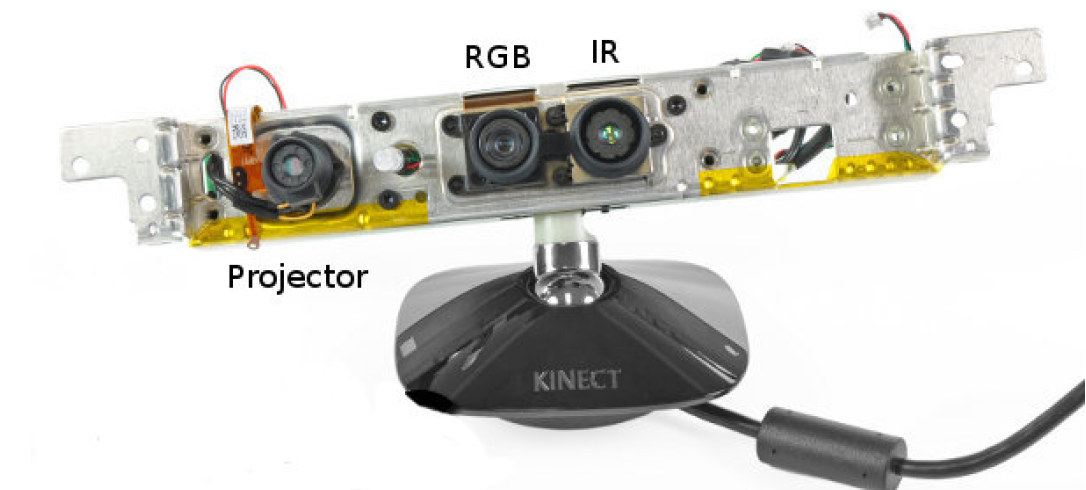
\includegraphics[width=0.5\linewidth]{figs/kinect.png}
	\caption{%
	Imagem de um Kinect V1 aberto, constituído de uma câmera infra-vermelho (IR - \emph{Infra-Red}), uma câmera RGB e um projetor IR.
	\protect\cite{smisek20133d}.
	}\label{fig:kinectv1}
\end{figure}

\subsection*{Processo de calibração}

Sua principal saída da imagem do Kinect é correspondente à profundidade da cena. Em vez de providenciar uma profundidade $Z$, ele retorna uma profundidade inversa, $D$.
A profundidade da imagem é construída a partir da triangulação da imagem IR com o projetor e, consequentemente, "carregada" pela imagem IR.

\begin{figure}[!h]
	\centering
	%   \includegraphics[width=1.0\linewidth]{figs/3d-curve-sketch/system-diagram.eps}
	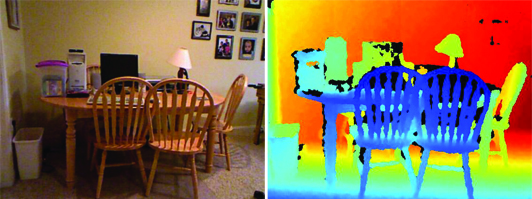
\includegraphics[width=1\linewidth]{figs/profundidadekinect.png}
	\caption{%
	Exemplo de como é a saída de uma imagem interpretada pelo Kinect, onde cada cor disposta na imagem, corresponde à profundidade ou distância da cena para o Kinect.
	\cite{Silberman:ECCV12}.
	}\label{fig:profKinect}
\end{figure}
 
Foram realizados alguns experimentos associando o uso do Kinect V1 como um escaneador em reconstruções. Primeiramente, foi executado uma calibração do Kinect para este tipo de reconstrução, onde a partir de experimentos, o sistema foi modelado como \ref{eq:kinectCalibracao}.

\begin{equation}
\label{eq:kinectCalibracao}
q(z)=2.73z^{2}+0.74z-0.58
\end{equation}

Onde "z" é a profundidade em metros, e "q" a quantização, em milímetros.

O modelo geométrico do Kinect foi criado com um sistema \emph{multi-view} considerando o RGB, IR e a profundidade.

\begin{gather} 
\label{eq:matrix}
\begin{bmatrix}
u\\
v\\
1
\end{bmatrix} 
= K
\begin{bmatrix}
s\\
t\\
1
\end{bmatrix}
\end{gather}

\begin{gather} 
\begin{bmatrix}
s\\
t\\
1
\end{bmatrix} 
= 
\underbrace{(1 + k_1r^2 + k_2r^4 + k_5r^6) 
\begin{bmatrix}
p\\
q\\
0
\end{bmatrix} }_{\text{distorção radial}} 
+
\underbrace{
\begin{bmatrix}
2k_3pq+k_4(r^2+2p^2)\\
2k_4pq+k_3(r^2+2q^2)\\
1
\end{bmatrix} }_{\text{distorção tangencial}}
\label{eq:distorcaoKinect}
\end{gather}

\begin{gather}
r^2 = p^2+q^2, 
\begin{bmatrix}
pz\\ 
qz\\ 
z
\end{bmatrix} = R(X-C)
\label{eq:relacaoKinect}
\end{gather}



Onde $k_n$ é o parâmetro de distorção, matriz de calibração da câmera $K$, rotação $R$ e centro $C$.

A profundidade é associada à geometria da câmera IR. que retorna a profundidade inversa ao longo do eixo $z$.

Os valores de $u$ e de $v$ são dados pela equação \ref{eq:distorcaoKinect} %(substitui-se o vetor [s, t, 1] em 2), X é o ponto coordenada 3D, c1 e c0 parâmetros do modelo.

\begin{gather} 
X_{IR} = \frac{1}{c_1 d + c_0}dis^{-1}\left ( K^{-1}_{IR}
\begin{bmatrix}
x+u_0\\ 
y+v_0\\ 
1
\end{bmatrix},k_{IR} 
\right )
\label{eq:distKinect}
\end{gather}

\begin{equation}
\label{eq:finalKinect}
u_{RGB} = K_{RGB} dis(R_{RGB}(X_{IR} - C_{RGB}),k_{RGB})
\end{equation}

Associamos o sistema de coordenadas do Kinect com a câmera IR e consequentemente, $R_{IR} = I$ (identidade) e $C_{IR} = 0$. 
O ponto 3D $X_{IR}$ é construído a partir da medição de [x,y,d] de \ref{eq:distKinect} e produz uma imagem RGB de \ref{eq:finalKinect}.

Em \ref{eq:distKinect}, $dis$ é a distorção, proveniente de \ref{eq:distorcaoKinect}, $k_{IR}$ e $k_{RGB}$ são, respectivamente, distorção relacionada à IR e à RGB. 
$K_{IR}$ é a matriz de calibração da câmera IR, $K_{RGB}$ é a matriz de calibração da câmera RGB. $R_{RGB}$ e $C_{RGB}$ são, a matriz de rotação e de centro da câmera RGB, respectivamente.

A calibração ocorreu usando o mesmo alvo nas câmeras IR e RGB, mesmos pontos 3D, e consequentemente, a mesma posição relativa das câmeras.
O sistema de coordenadas global do Kinect faz a posição relativa da câmera igual a $R_{RGB}$, $C_{RGB}$.

Também foi observado que existe um deslocamento entre imagem IR e a imagem da profundidade criada pelo Kinect. Para contornar este problema, uma série de experimentos foram executados, gerando \ref{tab:deslocamentoKinect}.

\begin{table}[!h]
\centering
\caption{Valores de deslocamentos e sua média}
\label{tab:deslocamentoKinect}
\begin{tabular}{|l|l|l|l|l|l|}
\hline
Imagem & 1   & 2   & 3   & 4   & Média \\ \hline
$u_0$  & 2,8 & 2,9 & 3,0 & 3,4 & 3,0   \\ \hline
$v_0$  & 3,0 & 2,7 & 2,8 & 3,1 & 2,9   \\ \hline
\end{tabular}
\end{table}

\begin{figure}[!h]
	\centering
	\subfloat[Sem o alinhamento]{\label{fig:deslocamentokinectA}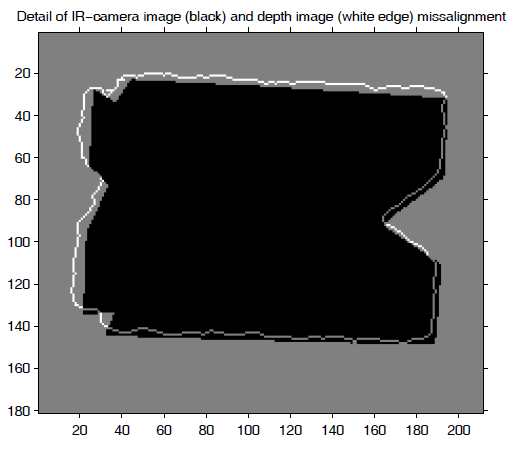
\includegraphics[width=0.3\linewidth]{figs/deslocamentokinectA.png}}
	\subfloat[Com o alinhamento]{\label{fig:deslocamentokinectB}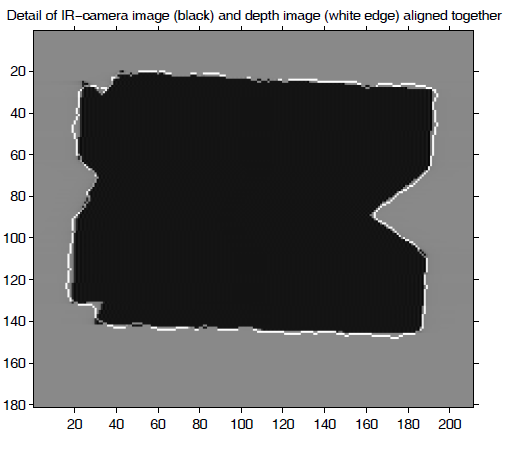
\includegraphics[width=0.3\linewidth]{figs/deslocamentokinectB.png}}
	\caption{%
	Representação visual do acerto do deslocamento. A parte em preto é a imagem IR e o contorno em branco é a imagem de profundidade do alvo.
	\protect\cite{smisek20133d}
	}\label{fig:deslocKinect}
\end{figure}

Foi observado que após a calibração, o Kinect gerava erros residuais complexos, que para compensar esse erro residual, foi criada uma correção em $z$, onde é subtraído da coordenada $Z_{IR}$ de \ref{eq:distKinect}.
Para validar essa correção, a correção-z das imagens foram construídas a partir dos resíduos das imagens ímpares e aplicadas nas pares, e o vice-versa. Depois da aplicação da correção-z , a media dos erros diminuiu aproximadamente 0,25mm.
Como parâmetro de comparação, foram dispostas 2 câmeras diferentes, no mesmo ambiente do Kinect.

\begin{figure}[!h]
	\centering
	%   \includegraphics[width=1.0\linewidth]{figs/3d-curve-sketch/system-diagram.eps}
	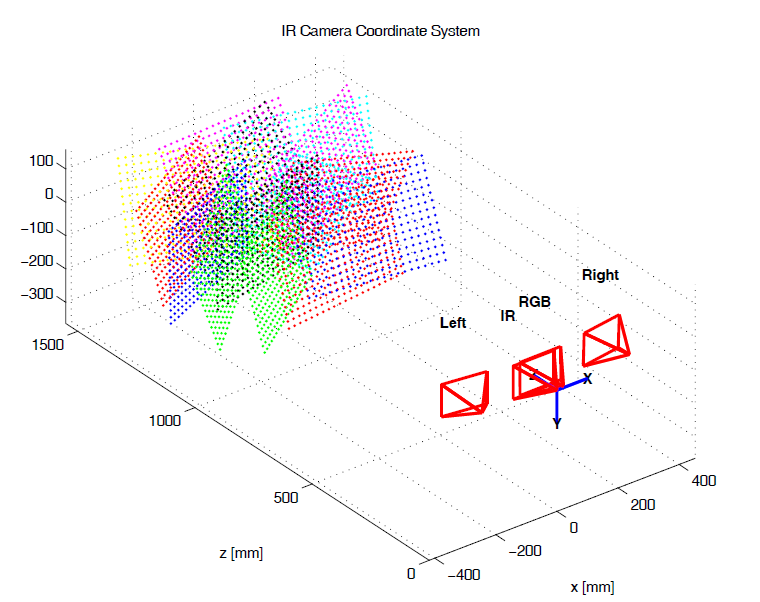
\includegraphics[width=0.5\linewidth]{figs/ambientekinect.png}
	\caption{%
	Posição e orientação do Kinect (com as câmeras IR e RGB) e o par estéreo SLR (\emph{Left}, \emph{Right}) em conjunto com pontos de calibração 3D reconstruídos em alvos de calibração planar.
	\protect\cite{smisek20133d}.
	}\label{fig:ambienteKinect}
\end{figure}

\begin{table}[htbp]
\caption{Resultados dos testes executados no ambiente descrito anteriormente}
\label{tab:resultadosKinect}
\begin{center}
\begin{tabular}{|c|c|c|c|}
\hline
\multirow{2}{1.5cm}{Método}& \multicolumn{3}{p{5cm}|}{Erro geométrico $e$ [mm]} \bigstrut \\
\cline{2-4} & \multicolumn{1}{c|}{$\mu$($e$)} & \multicolumn{1}{c|}{$\sigma$($e$)} & \multicolumn{1}{c|}{max($e$)} \bigstrut \\ \hline
SLR Stereo & 1,57 & 1,15 & 7,38 \bigstrut \\ \hline
Kinect & 2,39 & 1,67 & 8,64 \bigstrut \\ \hline
SR-4000 & 27,62 & 18,20 & 133,85 \bigstrut \\ 
\hline
\end{tabular}
\end{center}
\end{table}

\subsection*{Uso do Kinect com \emph{Structure from Motion}}

Com o sistema calibrado, o Kinect foi testado usando técnicas \emph{Structure from Motion}, onde a figura a seguir compara a superfície 3D de nuvem de pontos com uma com Kinect. 

O resultado é tão bom quanto ao mais acurado \emph{Multi-View Stereo}.

O Kinect tem a capacidade e, com o procedimento de calibração, é possível combiná-lo com técnicas \emph{SfM} e \emph{multi-view stereo}, o que abre uma nova aplicação na área de reconstrução 3D.

Quanto a qualidade da reconstrução de multi-view, o Kinect ficou melhor que o SR-4000 e perto do 3.5M SLR Stereo \ref{tab:resultadosKinect}.

%COLOCAR IMAGEM COMPARATIVA AQUI%
%\begin{figure}[!h]
%	\centering
%	\subfloat[Sem o alinhamento]{\label{fig:deslocamentokinectA}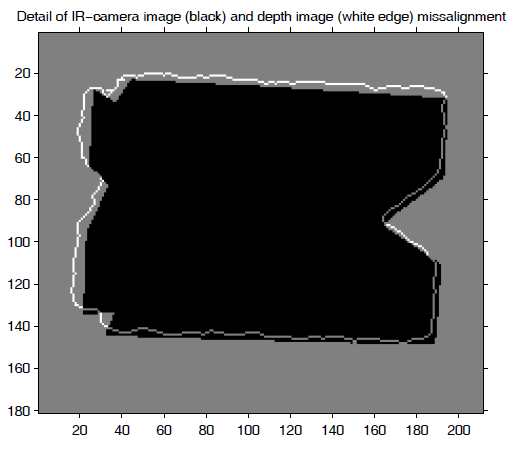
\includegraphics[width=0.3\linewidth]{figs/deslocamentokinectA.png}}
%	\subfloat[Com o alinhamento]{\label{fig:deslocamentokinectB}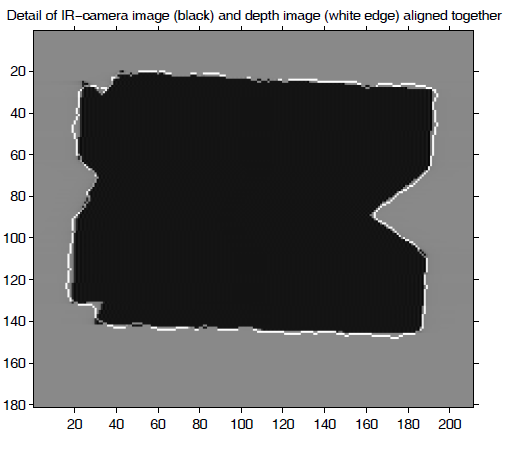
\includegraphics[width=0.3\linewidth]{figs/deslocamentokinectB.png}}
%	\caption{%
%	Representação visual do acerto do deslocamento. A parte em preto é a imagem IR e o contorno em branco é a imagem de profundidade do alvo.
%	}\label{fig:deslocKinect}
%\end{figure}

O Kinect é tão utilizado para fins pessoais (e empresariais), que existem alguns softwares para utilizá-lo como uma ferramenta de reconstrução 3D e a maioria deles são bem acessíveis (incluindo um pacote de ferramentas que a própria Microsoft disponibilizou, para o funcionamento do Kinect no Windows). Uma delas é o \emph{Skanect} que tem a versão gratuita onde é possível fazer escaneamentos básicos e a versão paga, que possibilita uma configuração maior, como por exemplo, a delimitação do objeto que será reconstruído, exportar o arquivo em diferentes formatos (\emph{.PLY}; \emph{.OBJ}: formato para exportação para programas que melhoram o modelo gerado (blender ou sculptris, por exemplo). E escolher o numero de faces a ser exportado; \emph{STL}: próprio para a impressora 3D (software \emph{Cura}); \emph{VRML}: salva também as cores do modelo.)

Entretanto, uma desvantagem que diminui a aplicabilidade do Kinect é que ele foi projetado para funcionar bem em espaços fechados, com detecção de formas humanas e movimentações. Ou seja, numa aplicação \emph{in situ} já não funcionaria muito bem, pois além de não conseguir projetar os detalhes em alta definição de uma escultura, ele necessita de uma fonte de energia externa, o que dificulta a acessibilidade, e, como  é gerada uma reconstrução em tempo real (não tem uma forma de salvar em \emph{cache} ou internamente), ele precisa estar ligado a um computador para fazer o escaneamento.
